\noindent

\includegraphics[height=1.25cm]{images/pictograms/replication}
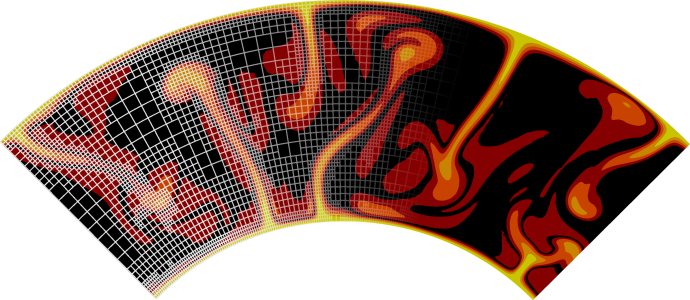
\includegraphics[height=1.25cm]{images/pictograms/aspect_logo}

\includegraphics[height=1.25cm]{images/pictograms/benchmark}

\includegraphics[height=1.25cm]{images/pictograms/under_construction}

\includegraphics[height=1.25cm]{images/pictograms/FEM}
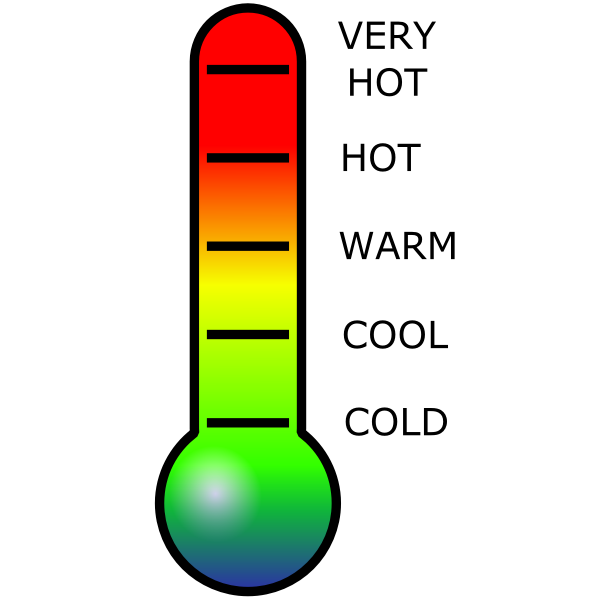
\includegraphics[height=1.25cm]{images/pictograms/temperature}

\includegraphics[height=1.25cm]{images/pictograms/paraview}

%%%%%%%%%%%%%%%%%%%%%%%%%%%%%%%%%%%%%%%%%%%%%%%%%%%%%%%%%%%%%%%%%%%%%%%%%%%%%%%%%%%%%%%%%%%%%%%%%%%

\begin{flushright} {\tiny {\color{gray} python\_codes/fieldstone\_168/text.tex}} \end{flushright}

%\lstinputlisting[language=bash,basicstyle=\small]{python_codes/template_keywords.key}

\par\noindent\rule{\textwidth}{0.4pt}

\begin{center}
\inpython
{\small Code: \url{https://github.com/cedrict/fieldstone/tree/master/python_codes/fieldstone_168}}
\end{center}

\par\noindent\rule{\textwidth}{0.4pt}

%%%%%%%%%%%%%%%%%%%%%%%%%%%%%%%%%%%%%%%%%%%%%%%%%%%%%%%%%%%%%%%%%%%%%%%%%%%%%%%%%%%%%%%%%%%%%%%%%%%

This is an attempt at replicating \fullcite{kiso20} with both a self-made Python code and the 
community code ASPECT.
When replicating a study I will always reproduce the abstract:
\begin{displayquote}
{\color{darkgray}
Edge-driven convection, which affects partial melting, intraplate volcanism, and dynamic topography, is small-
scale convection that occurs along a lithospheric keel with a sharp contrast in lithospheric thickness. Various
factors, including Rayleigh number, lateral mantle temperature heterogeneity, and geometry of the keel, 
influence the edge-driven convection, and the correlation between edge-driven convection and surface expressions
(dynamic topography and volcanism) is complicated. We performed a finite element study to quantify the effects
of these factors on dynamic topography and partial melting. We found that the dynamic topography is more
prominent when a strong edge-driven convection cell develops, which corresponds to homogeneous mantle
temperatures and the absence of mantle wind. In contrast, the development of edge-driven convection cells and
dynamic topography near the lithospheric keel are hindered when the mantle temperature is strongly 
heterogeneous (laterally varying $\sim$280 K). This indicates that a large lateral contrast 
in mantle temperature results in a
strong mantle wind that may prevent the development of edge-driven convection cells. An increase in the
Rayleigh number results in more vigorous convection and enhances partial melting. Our study shows that the
location of volcanic activity at craton edges and passive margins can be reproduced in models with weakly
heterogeneous mantle temperature for given mantle viscosity. The existence of a strong mantle wind (e.g.,
related to subducting slabs or mantle plumes) may inhibit the formation of an edge-driven convection cell and its
related partial melt near a lithospheric keel. However, mantle conditions with weak temperature heterogeneity
($< \sim 14$ K) or high mantle viscosity ($> 17\times 10^{19}~\si{\pascal\second}$), which corresponds 
to the Rayleigh number of $1.8\times 10^6$,
do not induce partial melts despite the development of edge-driven convection cells. Our model parametrized the
condition and location of edge-driven convection cells and partial melts, which can contribute to understanding
anomalous intraplate volcanisms, such as in Jeju Island south of the Korean Peninsula and the Tanzania Craton
near the East African Rift.}
\end{displayquote}

%===================================
\section*{The setup}

I then proceed to thoroughly read the paper in order to extract all what is needed to setup 
the experiment. 
The authors present the following equations after explaining that all quantities in these
are dimensionless:
\begin{center}
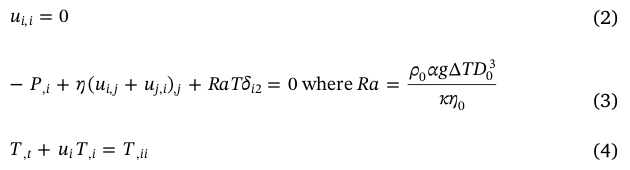
\includegraphics[width=9cm]{python_codes/fieldstone_168/images/kiso20c.png}
\end{center}
with the following table of parameters:
\begin{center}
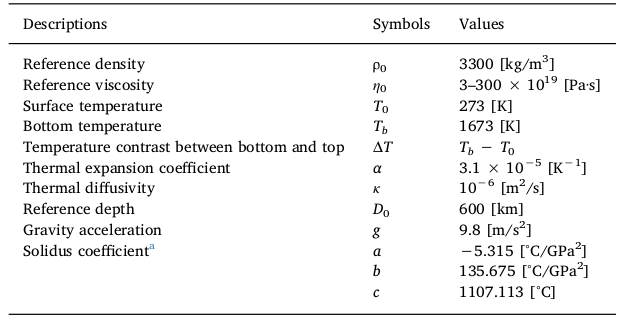
\includegraphics[width=9cm]{python_codes/fieldstone_168/images/kiso20a.png}
\end{center}
We also find a setup figure that shows the geometry, 
boundary conditions, initial temperature, etc ...
\begin{center}
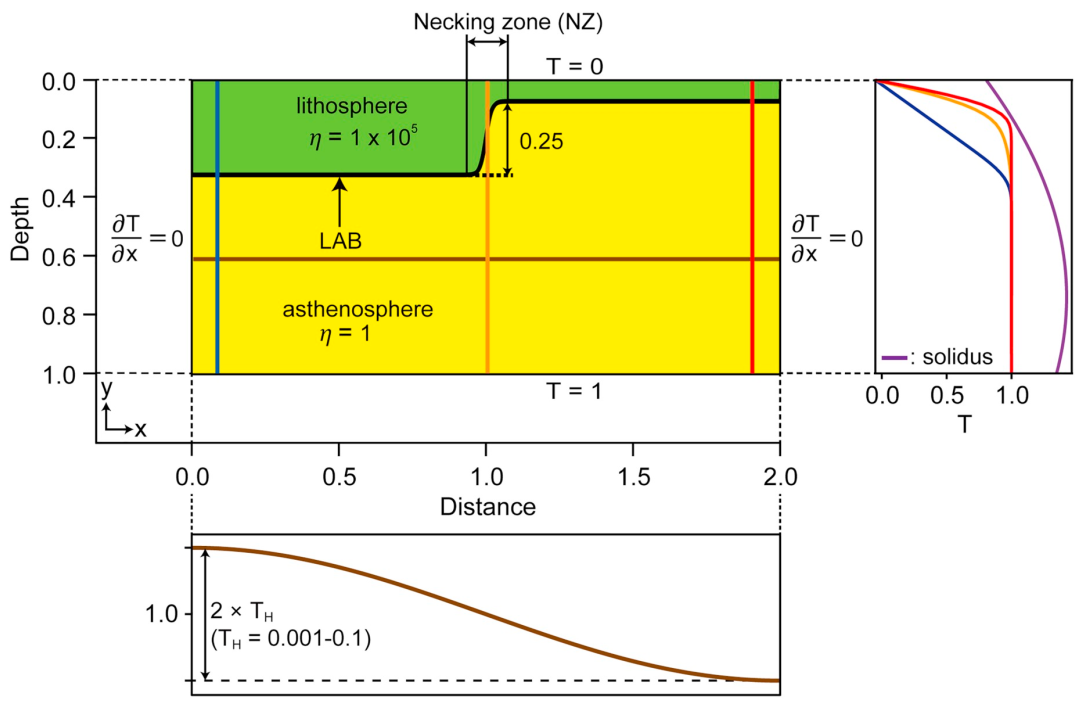
\includegraphics[width=11cm]{python_codes/fieldstone_168/images/kiso20b.png}
\end{center}

In the text we further find: $L_x=1200~\si{\km}$ and $L_y=600~\si{\km}$.
The lithospheric thickness decreases from
0.333 (200~\si{\km}) to 0.083 (50~\si{\km}) through the necking zone with a finite
width (i.e., NZ).
Most of the numerical models in the paper use a lithospheric
geometry with NZ=30~\si{km}. However, other lithospheric geometries 
with NZ=1200~\si{\km} and 300~\si{\km} were tested to
explore the effect of NZ on EDC (edge-driven convection) cell generation.

The viscosity of lithosphere is $10^5$ times that of the asthenosphere.
All viscosities are linear and temperature independent (although 
later on in the paper the authors explore temperature-dependent viscosities).
The authors use $\Ranb$ values from $10^5$ to
$10^7$ by controlling mantle viscosity from $300\cdot 10^{19}~\si{\pascal\second}$ to
$3\cdot 10^{19}~\si{\pascal\second}$, respectively. Radiogenic and adiabatic heating within
the crust are ignored.


The thermal boundary conditions of the model are $T_t=273$ K
and $T_b=1673$ K for the top and bottom temperatures
and from the figure we see that no heat-flux boundary conditions are
prescribed on the sides.
The initial temperature was set to 1673~K along and below the LAB
(thick black line on the figure above).
In order to explore the effect of long-wavelength thermal heterogeneity 
on EDC ithe authors add a background temperature heterogeneity 
so that the temperature in the asthenosphere is given by:
\[
T(x,y)=T_b + T_H \sin\left(\frac{\pi y}{L_y}\right) \cos \left(\frac{\pi x}{2 L_y} \right)
\]
where $T_H\in \{0.1,0.01,0.001 \}\cdot 1400~\si{\kelvin}$ 
refers to the magnitude of temperature heterogeneity.

The temperature field inside the lithosphere is shown in the right 
insert of the figure above but its exact expression is not specified,
nor how it is prescribed inside the necking zone.
All we know is that ``A thicker lithosphere has a
more gradual geothermal gradient than a thinner lithosphere''.

Based on the equations, and in the absence of a $Rb$ number in the rhs (e.g. \cite{chsg14})
that accounts for the different buoyancy of the materials in the domain, 
we will assume that both lithosphere and asthenosphere have the same density $\rho_0$
and thermal expansion coefficient $\alpha$.
From the equations above we can infer that the authors use the Boussinesq 
approximation, with $\rho(T)=\rho_0(1-\alpha T)$ in the rhs of the momentum equation.

When it comes to the boundary conditions for the Stokes equations, 
we read ``We did not impose any kinematic boundary condition for driving mantle convection'',
which (also based on the figures) probably means that free slip
boundary conditions are imposed on all sides.

The authors solve the equations with the commercial code COMSOL.
The finite element method is used with $Q_2\times Q_1$ elements for velocity and
pressure respectively and $Q_2$ elements are used for temperature.
They use a resolution of 5~\si{\km}, so that there are $240\times 120$ elements
in the domain\footnote{We read in the paper: ``The domain for numerical simulation was 
divided by $241\times 121$ grids in the horizontal and vertical directions, respectively''.
This obviously makes little sense. Also the mesh would then consist of $481\times 241$
velocity nodes, not $241\times 121$.}.

\vspace{1cm}

Open questions:
\begin{enumerate}
\item Do both lithosphere and asthenosphere have the same density?
\item What is the exact shape of the LAB. How is it parameterised?
\item How is the initial temperature inside the lithosphere prescribed?
\item Is the perturbation with the $T_H$ term applied {\it everywhere} in 
the asthenosphere? 
\item The temperature perturbation is not zero on the LAB, which renders the 
initial temperature field discontinuous there. Is this not a problem?
\item What is not clear from the setup in the paper is whether or not the lithosphere 
deforms with time. We know that time stepping is carried out (temperature is advected,
the $v_{rms}$ evolves with time), but if the lithosphere also deforms with the flow, 
what is the technique employed? particle-in-cell? compositional fields?
\end{enumerate} 


%===================================
%\section*{My implementation}




